\documentclass[tikz,border=2pt]{standalone}
\usepackage{amsmath}
\usepackage{pgfplots}
\pgfplotsset{compat=1.18}
\usetikzlibrary{arrows.meta}
\begin{document}
% At constant force 0.1, {}_tp_x = e^{-0.1t}: the area under the curve is the complete expectation 10;
% the unit-width bars of height {}_kp_x (k = 1,2,...) sum to the curtate expectation 1/(e^{0.1}-1) ~ 9.508.
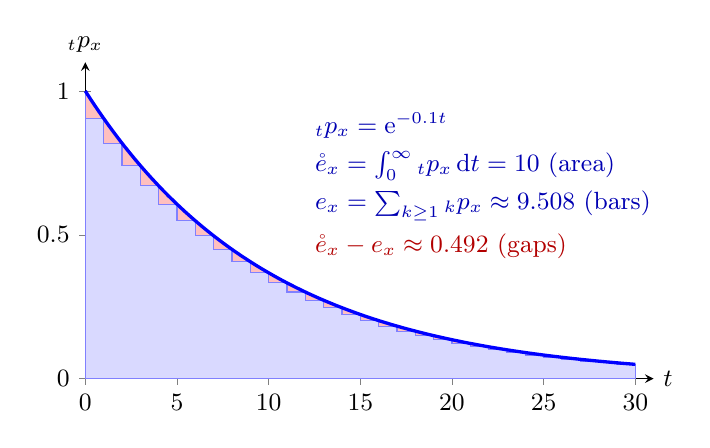
\begin{tikzpicture}[font=\small, >={Latex[length=2mm]}]
  \begin{axis}[
    axis lines=left, xmin=0, xmax=31, ymin=0, ymax=1.1,
    xtick={0,5,10,15,20,25,30}, ytick={0,0.5,1},
    xlabel={$t$}, ylabel={${}_tp_x$},
    xlabel style={at={(axis description cs:1,0)}, anchor=west},
    ylabel style={rotate=-90, at={(axis description cs:0,1)}, anchor=south},
    width=8.8cm, height=5.6cm, clip=false]
    \addplot[fill=red!25, draw=none, domain=0:30, samples=100] {exp(-0.1*x)} \closedcycle;
    \addplot[fill=blue!15, draw=blue!50, thin, const plot mark right, samples at={0,1,...,30}] {exp(-0.1*x)} \closedcycle;
    \addplot[blue, very thick, domain=0:30, samples=100] {exp(-0.1*x)};
    \node[blue!70!black, anchor=west] at (axis cs:12,0.88) {${}_tp_x=\mathrm{e}^{-0.1t}$};
    \node[blue!70!black, anchor=west] at (axis cs:12,0.74) {$\mathring e_x=\int_0^\infty{}_tp_x\,\mathrm{d}t=10$ (area)};
    \node[blue!70!black, anchor=west] at (axis cs:12,0.6) {$e_x=\sum_{k\ge1}{}_kp_x\approx9.508$ (bars)};
    \node[red!70!black, anchor=west] at (axis cs:12,0.46) {$\mathring e_x-e_x\approx0.492$ (gaps)};
  \end{axis}
\end{tikzpicture}
\end{document}
